\originalchapter{习题课十一: 干涉与衍射}
题源为\href{https://ocw.mit.edu/courses/8-02-physics-ii-electricity-and-magnetism-spring-2007/resources/solving11/}{Problem Solving 11}, PDF第1--12页. Q1--Q12全部保留, 答题页重复题干不再重复. 所有解答为AI独立解答.

\begin{exercise}
两窄缝相距$d$, 在$x=0$平面, 屏在$x=D$, 上缝编号1、下缝编号2. $O$是缝中点向屏作垂线的足点, 正$y$向上, 屏上$P$距$O$的有符号距离为$y$, $\theta$从正$x$轴量到缝中点指向$P$的射线. 两束同频、同偏振、相干的光从缝同相出发, 每束场幅度$E_0$. 第2缝到$P$比第1缝路长$\delta=r_2-r_1$. 采用远场近似.
Q1画两列相加增强的行波.
Q2画两列相加相消的行波.
Q3说明$\delta=m\lambda$为何增强.
Q4由双缝几何说明增强条件$d\sin\theta=m\lambda$.
Q5解释相消条件$d\sin\theta=(m+1/2)\lambda$.
Q6求亮纹$y$与$\lambda,d,D$关系.
Q7求暗纹位置关系.
Q8说明$\phi=2\pi d\sin\theta/\lambda$.
Q9设$E_1=E_0\sin\omega t,E_2=E_0\sin(\omega t+\phi)$, 用和差恒等式求总场.
Q10说明$I=I_{\max}\cos^2(\phi/2)$在何时最大.
Q11在$D\gg d\gg\lambda$下画随$y$变化的强度.
Q12因为能量与场平方有关, 是否有$\langle(E_1+E_2)^2\rangle=\langle E_1^2\rangle+\langle E_2^2\rangle$? 能量是否守恒?
\end{exercise}
\begin{solution}
Q1--2. 同相同幅相加幅度加倍, 相差$\pi$时逐点相消. 下图上行画同相两波(用不同线型区分), 下行画反相两波; 横轴是同一时刻沿传播方向的位置.
\begin{center}\begin{tikzpicture}\begin{axis}[width=.65\linewidth,height=3.5cm,xlabel={相位位置},ylabel={$E/E_0$},xmin=0,xmax=6.283,ymin=-1.4,ymax=1.4,xtick={0,3.14159,6.283},xticklabels={0,$\pi$,$2\pi$},ytick={-1,0,1}]
\addplot[thick,domain=0:6.283,samples=120]{sin(deg(x))};\addplot[dashed,main,domain=0:6.283,samples=120]{sin(deg(x))};
\end{axis}\end{tikzpicture}
\begin{tikzpicture}\begin{axis}[width=.65\linewidth,height=3.5cm,xlabel={相位位置},ylabel={$E/E_0$},xmin=0,xmax=6.283,ymin=-1.4,ymax=1.4,xtick={0,3.14159,6.283},xticklabels={0,$\pi$,$2\pi$},ytick={-1,0,1}]
\addplot[thick,domain=0:6.283,samples=120]{sin(deg(x))};\addplot[dashed,main,domain=0:6.283,samples=120]{-sin(deg(x))};
\end{axis}\end{tikzpicture}\end{center}
Q3. 多走一波长多积累$2\pi$相位, 整数波长使峰谷同步, $m=0,\pm1,\ldots$.
Q4. 远处到两缝的射线近似平行, 把缝距投影到传播方向即得$\delta\simeq d\sin\theta$, 因而亮纹条件如题.
Q5. 半整数波长使一束峰对应另一束谷, 相位差为奇数倍$\pi$, 同幅同偏振时完全相消.
Q6--7. 几何上$y=D\tan\theta$. 若还取小角度, 亮纹$y_m\simeq m\lambda D/d$, 暗纹$y_m\simeq(m+1/2)\lambda D/d$. 若不取小角度, 分别令$s=m\lambda/d$或$s=(m+1/2)\lambda/d$, 用$y=Ds/\sqrt{1-s^2}$, 要求$|s|<1$.
Q8. 相位与路程各绕一周期的比值相等,$\phi/(2\pi)=\delta/\lambda$, 得所问关系. 原题把延迟写成正$\phi$是相位约定, 强度只含$\cos^2(\phi/2)$, 改取负延迟不会改变强度.
Q9. 由$\sin A+\sin B=2\sin[(A+B)/2]\cos[(A-B)/2]$, 得$E_{\rm total}=2E_0\sin(\omega t+\phi/2)\cos(\phi/2)$.
Q10. 周期平均场平方为$2E_0^2\cos^2(\phi/2)$, 最大当$\phi=2\pi m$, 即$d\sin\theta=m\lambda$.
Q11. 在小角度区$I(y)/I_{\max}=\cos^2[\pi y/(\lambda D/d)]$, 中央亮纹是$y=0$, 相邻亮纹间隔$\lambda D/d$.
\begin{center}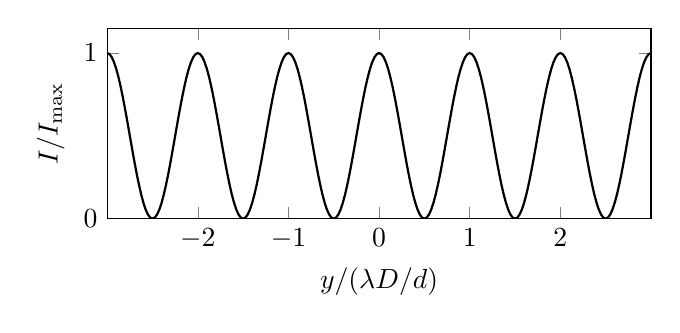
\begin{tikzpicture}\begin{axis}[width=.7\linewidth,height=4cm,xlabel={$y/(\lambda D/d)$},ylabel={$I/I_{\max}$},xmin=-3,xmax=3,ymin=0,ymax=1.15,xtick={-2,-1,0,1,2},ytick={0,1}]
\addplot[thick,domain=-3:3,samples=241]{cos(deg(pi*x))^2};
\end{axis}\end{tikzpicture}\end{center}
Q12. 一般不相等, 因为交叉项$2\langle E_1E_2\rangle=E_0^2\cos\phi$并非零. 这不是能量不守恒; 该等式比较的是单点局部强度, 干涉把能量分配到别的方向与位置. 对足够覆盖完整条纹的屏面积和完整源系统, 功率输入与输出仍由坡印廷定理约束. 相位随机化时交叉项平均为零, 才退回两强度相加.
\end{solution}
